%==============================
%generovani

\chapter{Generování grafického obsahu}\label{chap:generovani}
Jak již bylo řečeno v předcházející kapitole, generování grafického obsahuje je pro intra klíčové.
Generují se textury, generují se modely, generuje se geometrie.
Generuje se rozmístění modelů ve scéně.
Generování grafických objektů sebou přináší výhody malé velikosti a parametrizování generování.
Můžeme si tedy například uložit jednu šablonu stromu a vhodným měněním parametrů generovat pokaždé jiný strom.
Nevýhodou generování je delší nahrávací čas.
Vytvoření kvalitní textury může být časově velmi náročné, z tohoto důvodu mívají intra delší inicializační časy.

%==============
%sum

\section{Šum}\label{sec:sum}
Šum je náhodný signál.
Se šumem se často setkáváme v elektronice.
Zde se jedná o nežádaný jev, který zkresluje výsledky.
Setkáváme se s ním také u digitálních fotografii, kde se například projevuje jako změna hodnoty daného pixelu.
V informatice se však šum využívá (například jako zdroj náhodných čísel).
Náhodná čísla (skutečně náhodná čísla) se využívají v kryptografii.
Běžně většinou nemáme k dispozici generátory skutečně náhodných čísel (je k tomu obvykle potřeba specializovaný hardware), proto se používají kongruentní generátory produkující pseudonáhodná čísla.
Seznam hodnot vygenerovaných tímto generátorem je pak považován za šum.
V počítačové grafice se setkáváme s různými druhy generátorů šumu založených na různých druzích generátorů pseudonáhodných čísel.
Na generátory čísel je kladena řada požadavků z pohledu statistiky.
Tyto požadavky je nutné dodržet v případech, kdy hrají důležitou roli (například v simulacích).
V počítačové grafice si však často vystačíme i s jednoduchými implementacemi.
U inter hraje nejdůležitější roli velikost a rychlost.

\subsection{Generátory pseudonáhodných čísel}
Existuje vícero druhů generátorů.
Některé v podobě kongruentního generátoru, jiné v podobě funkce, která má vstupní parametry a vždy pro stejné nastavení parametrů produkuje stejný pseudonáhodný výstup.
Tyto generátory produkují celočíselný výstup s ur\-či\-tým rozsahem.
Je vhodné generátory upravit tak, aby vracely čísla s plovoucí řádovou čárkou v rozsahu $\langle 0,1 \rangle$.
S tímto rozsahem se pak později lépe pracuje.
\begin{itemize}
\item
Kongruentní generátor.
U kongruentního generátoru se vyskytuje inicializační hodnota (takzvané semínko).
Generátor na základě tohoto semínka vygeneruje novou hodnotu a tu do semínka uloží.
Lineární kongruentní generátor má tvar $x_{n+1}=(a \cdot x_n+b) \% m$, kde $a,b,c$ jsou vhodně zvolené konstanty.
Semínko je pak $x_0$.

\item
Generátor založený na funkci.
Tento typ generátoru vrací stejná čísla na základě stejných celočíselných vstupů.
Nalezení takové funkce může být obtížné.
Základem je operace zbytku po celočíselném dělení ($\%$), která se při generování náhodných čísel často používá.
Tvar této funkce, kterou jsem v práci použil je $f(x)=(x^5+x^4+x^3+x^2+x^1) \% N$.
Číslo $N$ je hodnota $2^n,n>0$.
Tento zápis lze pomocí Hornerova schématu zefektivnit: $f(x)=(x(x(x(x(x+1)+1)+1)+1)) \% N $.
Pro vyčíslení jedné hodnoty potřebujeme jen čtyři násobení, čtyři sčítání a jednu operaci modulo.
Experimentálně jsem si ověřil, že pro $N=2^{24}$ funkce vrací pro vstup $x \in \langle 0,N-1 \rangle$ pokaždé jinou hodnotu.
Tento poznatek bychom mohli využít pro konstrukci inverzní funkce.
\end{itemize}

\subsection{Perlinův šum}
\label{subsec:perlin}
Perlinův šum posaný v \cite{KENPERLIN} a v \cite{HUGOPERLIN} je šum založený na šumové funkci.
V počítačové grafice se hojně využívá.
Perlinův šum vrací pro stejné souřadnice stejnou hodnotu v rozsahu $\langle -1,1 \rangle$.
Výsledná hodnota šumu na daných souřadnicích je získána jako součet šumových funkcí o různých frekvencích a amplitudách.
Frekvence se obvykle volí jako násobek základní frekvence $f_0$ mocninou dvě.
Amplituda jednotlivých frekvencí je určena počáteční amplitudou a perzistencí.
Pokud bychom zvolili počáteční amplitudu $A=1$, perzistenci $P=1/2$, tak pro frekvenci $f_0 \cdot 2^n$ je amplituda $a=A \cdot P^n$.
Perlinův šum budeme používat pro generování skyboxů.


\section{Generování šumu půlením intervalu}
Kdybychom vygenerovali sérii hodnot pomocí generátoru náhodných čísel, získali bychom šum, který není pro grafiku příliš vhodný.
Můžeme jej vidět v levé části obrázku \ref{fig:sum}.
Tento šum má hodnoty v sousedních bodech příliš odlišné.
Pro další generování (například textur) je tedy vhodné šum generovat jinak.
Důležité je, aby rozdíly v sousedních bodech byly malé.
Jedním ze způsobů jak to zajistit, je generovat hodnoty s ohledem na již vygenerované hodnoty.
Další vlastností, kterou chceme zaručit je, aby šum na sebe navazoval.
Toto lze zajistit algoritmem půlení intervalu, jehož výsledek je v pravé části obrázku \ref{fig:sum}.
Jak je z tohoto obrázku patrné, šum produkovaný tímto algoritmem je vhodnější pro další generování (například mraků).
\begin{figure}[h]
\centering
\includegraphics[width=7.5cm,keepaspectratio]{obr/simply_noise.png}
\includegraphics[width=7.5cm,keepaspectratio]{obr/midpoint_noise.jpg}
\caption{Vlevo: šum jako prostá sekvence náhodných čísel. Vpravo: šum vygenerovaný algoritmem půlení intervalu.}
\label{fig:sum}
\end{figure}

Generování šumu pomocí půlení intervalu je dopodrobna popsáno v bakalářské práci \cite{MILET}.
Základem je generátor čísel (v podobě kongruentního generátoru).
Předpokládejme, že chceme vygenerovat jednorozměrný šum reprezentovaný polem o $N$ prvcích s indexy $0,1,\dotsc,N-1$.
Máme k dispozici základní rozsah generátoru $d$ a faktor vyhlazování $m$.
Algoritmus pracuje následovně (jeho vizualizace je v levé části obrázku \ref{fig:midpoint} a výstup v pravé části obrázku \ref{fig:midpoint}):
\begin{enumerate}
\item
Nejprve se vygeneruje náhodná hodnota s rozsahem generátoru $\langle -d,d \rangle$ a uloží se do prvku s indexem $0$.

\item \label{itm:puleni}
Nastaví se nový rozsah $d:=d/m$.

\item
Určí se index $S$ vhodného středu. Je to největší možné číslo $2^n$ takové, že je menší než počet prvků pole ($N$).

\item \label{itm:stred}
Prvek s indexem $S$ má hodnotu součtu váženého průměru a nově vygenerované hodnoty s upraveným rozsahem.
Vážený průměr je počítán z hodnot nejbližších, již vygenerovaných prvků zleva a zprava od $S$, přičemž hodnota váhy je určená vzdáleností jejich indexů od $S$.
Čím je prvek od $S$ vzdálenější, tím má jeho hodnota menší váhu.
Součet vah je roven $1$.
Pokud žádný vygenerovaný prvek zprava neexistuje, použije se prvek s indexem $0$ a vzdálenost je spočítána jako vzdálenost k poslednímu prvku pole plus jedna.
Tímto je zajištěno opakování.

\item
Krokem \ref{itm:stred} nám vznikla dvě pole: jedno s indexy $0,\dotsc,S$ a druhé s indexy $S,\dotsc,N-1$.
Na tato pole se aplikuje tento algoritmus znovu od kroku \ref{itm:puleni}.
Pole však musí mít více než dva prvky.
\end{enumerate}

\begin{figure}[h]
\centering
\includegraphics[width=15cm,keepaspectratio]{obr/midpoint.pdf}
\caption{Vlevo: kroky algoritmu půlení intervalu. Vpravo: výsledek algoritmu půlení intervalu.}
\label{fig:midpoint}
\end{figure}

Výše popsaný postup je určen pro jednorozměrný šum.
Více rozměrná varianta je obdobná.
Výpočet hodnoty středního bodu se například pro dvojrozměrný šum nepočítá ze dvou ale ze čtyř okolních bodů.
Podrobně je obecný algoritmu popsán v bakalářské práci \cite{MILET}.


\section{Více dimenzí}
Jelikož se v této práci často pracuje s vícerozměrnými daty (příkladem může být výše zmíněný vícerozměrný šum), předvedeme si zde i postup, jak s těmito daty jednotně pracovat.
Vícerozměrná data budeme reprezentovat jednorozměrným seznamem (polem) prvků.
Způsob uspořádání prvků vícerozměrných dat do jednorozměrného seznamu je ukázán na obrázku \ref{fig:dimenze}, kde je předvedeno uspořádání trojrozměrných dat.
Index do $d$ rozměrného pole $I=(i_1,i_2,\dotsc,i_d)$ se skládá z $d$ složek (čísel) $i_n$, z nichž každé indexuje jinou dimenzi (složka $i_1$ nejnižší a složka $i_d$ nejvyšší).
Rozměry (výška, šířka, ...) dat označme $r=(r_1,r_2,\dotsc,r_d)$.
Přepočet na index $J$ do jednorozměrného pole je dán vztahem:
\begin{equation}
\label{eq:index}
J=i_1 + i_2 \cdot r_1 + i_3 \cdot r_1 r_2 + \dotsc = \sum_{k=1}^{d}\left(i_k \prod_{h=1}^{k-1}r_h \right)
\end{equation}
Vztah \ref{eq:index} můžeme zefektivnit a převést na rekurentní vztah:
\begin{eqnarray*}
\label{eq:fastindex}
J_1 &=& i_d \\
J_n &=& J_{n-1} \cdot r_{d-n+1} + i_{d-n+1} \\
J   &=& J_d
\end{eqnarray*}

\begin{figure}[h]
\centering
\includegraphics[width=5cm,keepaspectratio]{obr/dimenze.pdf}
\caption{Uspořádání 3D dat}
\label{fig:dimenze}
\end{figure}

%===========
%voronoid

\section{Voroného diagram}\label{sec:voronoid}
Voroného diagram popsaný v \cite{VORONOID} je způsob dekompozice metrického prostoru.
Dekompozice je určena vzdálenostmi k dané diskrétní množině objektů v prostoru, například diskrétní množinou bodů.
V levé části obrázku \ref{fig:voronoid} můžeme vidět příklad rozdělení dvourozměrného prostoru.
Pro rozdělení byla použita množina náhodných bodů (reprezentovány černými tečkami).
Jednotlivé barevné oblasti patří k danému černému bodu, který se v nich nachází.
Všechny body z jedné barevné oblasti mají společnou vlastnost: vzdálenost k černému bodu ležící v této oblasti je menší než vzdálenost ke všem ostatním černým bodů.
Matematicky si můžeme, pro naše potřeby, Voroného diagramy popsat následovně: mějme metrický prostor $(M,\rho)$ dimenze $d$, který reprezentuje všechny body Voroného diagramu.
Zobrazení $ \rho: M \times M \to \mathbb{R} $ je v našem případě Eulerova vzdálenost.
Dále mějme množinu indexů $K$ a body $P_k \in M, k \in K$.
Oblast (nebo buňka) Voroného diagramu, která je asociována k bodu $P_k$ označme množinou $R_k$.
Pak jsou body v jedné množině dány vztahem $R_k=\left\{ x \in M | \forall i \in K \setminus \{k\}: \rho(x,P_k) \leq \rho(x,P_i) \right\}$.
Počet buněk diagramu je $|K|$.

Využití Voroného diagramu může být například v texturách nebo při generování geometrie.
Voroného diagramy dělí prostor na buňky, proto poskytují dobrý základ k buněčným texturám.
Příkladem může být textura dlažby nebo textura vysušené půdy.

Aby se s diagramem dobře pracovalo je vhodné jej převést na normalizované vzdálenostní.
Vzdálenostní pole můžeme vidět v pravé části obrázku \ref{fig:voronoid}.
Každý prvek pole (pixel textury) si místo příslušnosti do dané oblasti nese informaci o normalizované vzdálenosti ke středu oblasti do které patří.
Pro výpočet vzdálenosti použijeme Eulerův výpočet vzdálenosti pro dimenzi prostoru $d$:

\begin{equation}
\label{eq:eulerovavzdalenost}
\rho(x,y)=\sqrt{\sum_{k=1}^{d}(x_k-y_k)^2}
\end{equation}

\begin{figure}[h]
\centering
\includegraphics[width=7.5cm,keepaspectratio]{obr/voronoid.pdf}
\includegraphics[width=7.5cm,keepaspectratio]{obr/vzdalenostni_pole.jpg}
\caption{Vlevo: Voroného diagram, Vpravo: vzdálenostní pole.}
\label{fig:voronoid}
\end{figure}

\subsection{Navazování}
Navazování Voroného diagramu a tedy i vzdálenostního pole, které je popsáno v \cite{VOROWEB} je důležitá vlastnost.
Aby se dala textura vytvořená na základě vzdálenostního pole použít opakovaně vedle sebe, je nutné zajistit navazování.
Navazování lze u vzdálenostního pole zajistit úpravou výpočtu vzdálenosti.
Označme $d$ dimenzí prostoru.
Bod v prostoru $x=(x_1,x_2,\dotsc,x_d)$.
Rozměry pole (výška, šířka, ...) označme $r=(r_1,r_2,\dotsc,r_d)$.
Předpokládejme, že všechny body vzdálenostního pole mají nezáporné souřadnice.
Upravený výpočet vzdá\-le\-nos\-ti \ref{eq:eulerovavzdalenost}, který respektuje navazování, je:

\begin{equation}
\label{eq:vorovzdalenost}
\rho'(x,y)=\sqrt{\sum_{k=1}^{d}\min(|x_k-y_k|,r_k-|x_k-y_k|)^2}
\end{equation}

Funkce $\min$ vrací minimum ze dvou hodnot.
Jak je z upraveného vypočtu patrné, absolutní velikost dílčího rozdílu $|x_k-y_k|$ nemůže být větší než $r_k/2$.
V případě, kdy je $|x_k-y_k|>r_k/2$ se použije pro výpočet bod, který leží v sousedním poli.
Sousední pole je totožné, jen je posunuté o $r_k$.
Názorně je to vidět na obrázku \ref{fig:navazovani}.

\begin{figure}[h]
\centering
\includegraphics[width=15cm,keepaspectratio]{obr/navazovani.pdf}
\caption{
Výpočet vzdálenosti.
Počítáme vzdálenost k bodu $X$.
Vzdálenost ke středu buňky $A$ v neopakujícím poli je $a=|XA|$.
Buňka, která je nejblíže k bodu $X$ v neopakujícím poli je $B$ (se vzdáleností $b=|XB|,b<a$).
V opakujícím poli je nejblíže bodu $X$ střed buňky $A'$, který je totožný s $A$ jen leží v posunutém poli.
Vypočítaná vzdálenost je tedy $a'=|XA'|$.}
\label{fig:navazovani}
\end{figure}

\subsection{Optimalizace}
Výpočet vzdálenostního pole je časově poměrně náročná záležitost.
Pro pole šířky $w$ a výšky $h$ a počtu buněk $b$ je potřeba provést $w \cdot h \cdot b$ výpočtů vzdáleností abychom zjistili nejmenší vzdálenost bodů ke středu buněk.
To znamená, z každého bodu pole spočítat vzdálenost ke všem středům buněk a vybrat tu nejmenší.
Kdybychom pro všechny body věděli, ke které buňce patří bylo by potřeba jen $w \cdot h$ výpočtů vzdáleností.
Optimalizací výpočtů se budeme snažit tomuto počtu výpočtů vzdáleností přiblížit.

Způsob, jak toho dosáhnout je rozmístit středy buněk do binárního stromu a počítat vzdálenosti jen k části stromu.
Binární strom má v každém uzlu dvojicí bodů.
Tato dvojice bodů dělí prostor na dvě části podle vzdálenosti k nim.
Vytvořit strom je snadné.
Nejprve se vytvoří kořenový uzel z prvních dvou středů buněk.
Poté se do stromu postupně přidávají další středy.
Pokud je nově vkládaný střed blíže k prvnímu bodu uzlu, vloží se do levého podstromu.
Pokud je blíže druhému bodu uzlu, vloží se do pravého podstromu.
Pokud podstrom neexistuje, vytvoří se nový uzel z dvojice, kterou tvoří nově vkládaný střed a první nebo druhý bod rodičovského uzlu.
Postupná tvorba stromu je znázorněna v levé části obrázku \ref{fig:vorostrom}.
Výsledný binární strom je pak v pravé části obrázku \ref{fig:vorostrom}.

\begin{figure}[h]
\centering
\includegraphics[width=15cm,keepaspectratio]{obr/vorostrom.pdf}
\caption{Vlevo: Postupné vkládání bodů do stromu. Vpravo: Výsledný strom}
\label{fig:vorostrom}
\end{figure}

Když máme vytvořený strom pro všechny středy buněk, je ještě potřeba spočítat k oběma bodům každého uzlu stromu vzdálenosti k nejvzdálenějším potomkům a ty do daného uzlu uložit.
Vzdálenosti jednotlivých bodů uzlů jsou znázorněny kružnicemi v levé části obrázku \ref{fig:vorokruh}.

Nalezení nejkratší vzdálenosti pro každý bod pole pak spočívá ve zvolení poloměru kolem zkoumaného bodu.
V prvním kroku zvolíme poměr jako vzdálenost ke středu náhodné buňky, pravá část obrázku \ref{fig:vorokruh}.
V dalších krocích budeme volit poloměr ze vzdálenosti ke středu poslední nejblíže nalezené buňky.
Pokud se kružnice kolem aktuálně zkoumaného bodu nepřekrývá s danou kružnicí v aktuálním uzlu, není třeba prohledávat jeho podstrom.
Pokud ano, prohledá se podstrom uzlu.
Pokud je vzdálenost k bodu uzlu menší než aktuální poloměr kolem zkoumaného bodu, zmenšíme poloměr na tuto vzdálenost.
Tím se nám neustále zmenšuje poloměr kolem zkoumaného bodu, než nalezneme hledanou vzdálenost.

\begin{figure}[h]
\centering
\includegraphics[width=7.5cm,keepaspectratio]{obr/vorokruh0.pdf}
\includegraphics[width=7.5cm,keepaspectratio]{obr/vorokruh1.pdf}
\caption{Vlevo: Kružnice kolem uzlů. Vpravo: Kružnice kolem zkoumaného bodu s poloměrem k náhodně vybrané buňce $D$.}
\label{fig:vorokruh}
\end{figure}


%=================
%textury

\section{Generování textur}
\label{sec:texture}
Textura slouží pro detailní popis struktury povrchu.
Vyskytují se nejčastěji ve formě dvojrozměrných obrázků.
Můžeme se ale setkat i s jednorozměrnými, trojrozměrnými nebo dokonce čtyřrozměrnými texturami.
Trojrozměrné textury slouží pro popis objemu a čtyř\-roz\-měr\-né pro popis objemu měnícího se v čase (například plameny ohně, kouř).
Textury si díky jejich velikosti nemůžeme do programu uložit, a tak je musíme generovat.
Vytvoření textury bývá obvykle časově náročné, neboť obsahují velké množství dat.
Základem pro vytvoření textur v této prací je šum, který je popsaný v části \ref{sec:sum} a vzdálenostního pole vytvořené z Voroného diagramu, který je popsaný v části \ref{sec:voronoid}.
Tyto dvě metody nám produkují $d$ rozměrné pole.
Všechny hodnoty těchto polí jsou v rozsahu $\langle 0,1 \rangle$.
Příklad šumu můžeme vidět v pravé části obrázku \ref{fig:sum} a příklad vzdálenostního pole v pravé části obrázku \ref{fig:voronoid}.
Nejdůležitějším vstupem algoritmu pro vytvoření šumu je faktor vyhlazení, který nám určuje poměr nízkých frekvencí a vysokých frekvencí ve výsledném šumu.
U Voroného diagramu je nejdůležitějším vstupem rozmístění a počet středů buněk.
Nicméně tyto možnosti nám neposkytují dos\-ta\-teč\-nou variabilitu textur.
Proto je vhodné pole hodnot produkované těmito postupy ještě dále upravit.
Upravit takové pole můžeme prostým obarvením pomocí barevného přechodu, globální transformací jako je například vyhlazení, lokální transformací a složením několika vstupů.
Jednotlivé úpravné operace si popíšeme v dalších částech práce.

\subsection{Barevné přechody}
Příklad barevného přechodu je zobrazen na obrázku \ref{fig:prechod}.
Barevný přechod (nebo též gradient) jsou v podstatě tři funkce $R(x),G(x),B(x)$ (čtyři v případě přítomnosti alfa kanálu).
Tyto funkce jsou definované na intervalu $\langle 0,1 \rangle$.
Jejich vstup je hodnota celkové intenzity barvy a výstupem intenzita červené respektive zelené respektive modré barvy.
Intenzity jsou taktéž v rozsahu $\langle 0,1 \rangle$.
Barevné přechody můžeme výhodně použít na obarvení obrázků v odstínech šedé.
Znázorněné to můžeme vidět na obrázku \ref{fig:gradmap}.
Pro uložení barevného přechodu stačí uložit jen kontrolní barvy a hodnoty mezi nimi interpolovat.
Například u barevného přechodu na Obrázek \ref{fig:prechod} stačí uložit pouze barvy: tmavě modrá, světle modrá, žlutá, světle zelená, tmavě zelená, šedá a bílá (v pořadí zleva doprava).
Tímto můžeme zredukovat paměťovou náročnost.
Další možností je vytvořit algoritmus na generování barevných přechodů.
Musíme však zvážit, jestli potřebujeme tolik různých barevných přechodů, že se nám je oplatí generovat.

\begin{figure}[h]
\centering
\includegraphics[width=15cm,keepaspectratio]{obr/gradient.png}
\caption{Barevný přechod, který je možné využít na obarvení výškové mapy.}
\label{fig:prechod}
\end{figure}

\begin{figure}[h]
\centering
\includegraphics[width=7.5cm,keepaspectratio]{obr/gradmap0.jpg}
\includegraphics[width=7.5cm,keepaspectratio]{obr/gradmap1.jpg}
\caption{Vlevo: vstupní obrázek v odstínech šedé. Vpravo: obarvený obrázek z leva barevným přechodem z obrázku \ref{fig:prechod}}
\label{fig:gradmap}
\end{figure}

\subsection{Globální transformace}
Globální transformací budeme v textu rozumět operaci, která transformuje vstupní $d$ roz\-měr\-né pole hodnot na výstupní $d$ rozměrné pole hodnot.
Pro výpočet jednoho prvku výstupního pole s indexem $I$ budeme potřebovat hodnoty okolí vstupního pole kolem indexu $I$.
Jedná se tedy o $d$ rozměrnou konvoluci s $d$ rozměrným konvolučním jádrem.
Pokud si vytvoříme obecnou konvoluci, můžeme ji použít pro řadu transformací.
Příkladem těchto transformací je vyhlazení a detekce hran.
Konvoluční jádro pro vyhlazení obsahuje hodnoty, které jsou všechny stejné a jejichž součet je roven jedné.

\subsection{Lokální transformace}
Lokální transformací budeme v textu rozumět (podobně jako globální transformace) operaci, která transformuje vstupní pole na výstupní pole hodnot.
Pole mají rozměr $d$.
Pro výpočet jednoho prvku výstupního pole s indexem $I$ budeme potřebovat několik hodnot ze vstupního pole.
Výběr těchto hodnot závisí na transformaci.
%Příklady lokálních transformací vzdálenostního pole můžeme vidět na Obrázek 3.15 až Obrázek 3.26.
Možnosti lokální transformace jsou velké.
Vše závisí na transformační funkci.
Důležité je, aby nám transformace zachovávala opakování.
Kdykoliv si transformace zažádá  hodnotu pole na souřadnicích, které leží mimo rozsah pole, budeme muset souřadnice přepočítat.
Souřadnice bodu pole je $I=(i_1,i_2,\dotsc,i_d)$ a velikost pole (výška, šířka, ...) je $r=(r_1,r_2,\dotsc,r_d)$.
Pokud je složka souřadnic $i_n<0 \vee i_n \geq r_n$ (hodnoty pole indexujeme od nuly), je potřeba ji přepočítat podle vztahu: $i'_n= ((i_n \% r_n)+r_n)\% r_n$.

V levé části obrázku \ref{fig:voropopis} můžeme vidět velmi jednoduchou transformaci.
K výpočtu výstupní hodnoty na souřadnicích $I=(i_1,i_2)$ jsou zapotřebí dvě hodnoty vstupního pole.
První hodnota vstupního pole, označme ji $a$ , je na totožných souřadnicích.
Druhá hodnota, označme ji $b$, je na souřadnicích $(i_1 + r\cdot \cos(2\pi a),i_2+r\cdot \sin(2\pi a))$.
Hodnota $r$ udává poloměr.
Hodnota $b$ je výsledná hodnota výstupního pole na souřadnicích $I$.
Můžeme vidět, že hodnota $a$ udává normalizovaný úhel.
Spolu s poloměrem $r$ vytváří vektor.
Když tento vektor přičteme k původním souřadnicím, máme souřadnice bodu, jehož hodnota je použita pro výstup – tedy hodnotu $b$.
Na dalších obrázcích je postup transformace obdobný.
V pravé části obrázku \ref{fig:voropopis} je výše popsaný postup opakován několikrát.
Místo abychom použili dva body ze vstupního pole, použijeme jich několik.
Poslední bod udává hodnotu výstupu.
Další příklady lokálních transformací můžeme vidět na obrázku \ref{fig:loctransform}

\begin{figure}[h]
\centering
\includegraphics[width=7.5cm,keepaspectratio]{obr/voro_00.jpg}
\includegraphics[width=7.5cm,keepaspectratio]{obr/voro_01.jpg}
\caption{Lokální transformace}
\label{fig:voropopis}
\end{figure}


\subsection{Skládání operací}
Nyní, když máme základ všech textur v podobě distančního pole a šumu, lokální a globální transformace a barevné přechody, můžeme se pustit do vytváření textur.
Vytvoření jedné textury si můžeme představit jako strom.
Uzly stromu představují operaci.
Operace uložena v uzlu bere své vstupy ze svých potomků a výstup posílá rodiči.
V listech tohoto stromu se nachází buď distanční pole nebo šum.
V uzlech stromu je lokální nebo globální transformace nebo jedna z následujících operací:
\begin{itemize}
\item
Součet hodnot vstupů.
\item
Rozdíl hodnot vstupů.
\item
Násobení hodnot vstupů.
\item
Součet hodnot vstupů s ohledem na alfa kanál.
\item
Kompozice vstupů do vícekanálové textury.
\end{itemize}
Příklad textury složené pomocí několika operací můžeme vidět na obrázku \ref{fig:slozenina}

\begin{figure}[h]
\centering
\includegraphics[width=7.5cm,keepaspectratio]{obr/slozeni.jpg}
\caption{Sestavená textura}
\label{fig:slozenina}
\end{figure}

\begin{figure}[htb]
\centering
\includegraphics[width=3cm,keepaspectratio]{obr/voro_02.jpg}
\includegraphics[width=3cm,keepaspectratio]{obr/voro_03.jpg}
\includegraphics[width=3cm,keepaspectratio]{obr/voro_04.jpg}
\includegraphics[width=3cm,keepaspectratio]{obr/voro_05.jpg}
\includegraphics[width=3cm,keepaspectratio]{obr/voro_06.jpg}
\includegraphics[width=3cm,keepaspectratio]{obr/voro_07.jpg}
\includegraphics[width=3cm,keepaspectratio]{obr/voro_08.jpg}
\includegraphics[width=3cm,keepaspectratio]{obr/voro_09.jpg}
\includegraphics[width=3cm,keepaspectratio]{obr/voro_10.jpg}
\includegraphics[width=3cm,keepaspectratio]{obr/voro_11.jpg}
\includegraphics[width=3cm,keepaspectratio]{obr/voro_12.jpg}
\includegraphics[width=3cm,keepaspectratio]{obr/voro_13.jpg}
\caption{Příklady lokálních transformací aplikovaných na vzdálenostní pole.}
\label{fig:loctransform}
\end{figure}



%===========
% geometrie

\section{Generování geometrie}
\label{sec:geometrie}

Pro generování geometrie můžeme použít několik postupů.
V práci budeme používat algoritmus, který převádí objemovou reprezentaci tělesa na povrchovou.
Pro vygenerování objemové reprezentace můžeme použít šum nebo vzdálenostní pole.
Můžeme použít také transformace (lokální, globální), které nám objemovou reprezentaci upraví.
Pro převod objemové reprezentace budeme používat algoritmus Marching tetrahedra.

\subsection{Převod do povrchové reprezentace}
V dnešní počítačové grafice se nejčastěji setkáme s povrchovou reprezentací těles.
Důvod je ten, že současný hardware je pro to optimalizovaný.
Občas je však vhodné specifikovat objekty objemem nebo pomocí implicitních ploch.
Příkladem je trojrozměrný šum, reprezentující hustotu objektu v daném místě prostoru.
Proto potřebujeme takto reprezentované objekty převést do povrchové reprezentace.
Existuje několik algoritmů pro převod.
Jedním z nejznámějších je Marching cubes.
Další používaný algoritmus je Marching tetrahedra.

\subsection{Marching cubes}
Marching cubes algoritmus popsán v \cite{MARCHINGCUBES} je v češtině algoritmus pochodujících krychlí.
Krychle stejné velikosti jsou pravidelně rozmístěny v prostoru, kde se nachází objekt, který chceme převést.
Abychom mohli algoritmus použít, musíme mít k dispozici funkci: $f: \mathbb{R}^3 \to \{0,1\} $.
Funkce zjistí, zda bod na daných souřadnicích leží uvnitř objektu (funkce vrací $1$) nebo vně (funkce vrací $0$).
Pro jednu krychli vyhodnotíme tuto funkci pro všechny její rohy.
Získáme jednu z $2^8$ možných ohodnocení rohů.
Existuje patnáct unikátních ohodnocení (konfigurací), které můžeme transformacemi převést na všechny ostatní.

\begin{figure}[h]
\centering
\includegraphics[width=15cm,keepaspectratio]{obr/mccase.pdf}
\caption{Unikátní konfigurace, obrázek převzat z \cite{MARCHINGCUBESCASE}}
\label{fig:mccase}
\end{figure}

Na hranách krychle se vyskytuje vrchol geometrie (trojúhelníku) v případě, kdy ohodnocení rohů krychle, které hrana sdílí, není stejné (na jednom rohu je $0$ a na druhém $1$).
Vznikne tak několik hran, na kterých leží vrcholy trojúhelníků.
Vhodným propojením vrcholů vznikne trojúhelníková síť pro jednu konfiguraci krychle.
Patnáct trojúhelníkových sítí pro patnáct unikátních konfigurací můžeme vidět na obrázku \ref{fig:mccase}.
Spojením všech trojúhelníkových sítí ze všech krychlí rozmístěných v prostoru vznikne výsledná síť.


Marching cubes algoritmus má jednu nevýhodu.
Některé konfigurace krychlí spolu nejsou kompatibilní podle \cite{MARCHINGCUBES}.
Pokud bychom nekompatibilní stavy neřešili, ve výsledné troj\-ú\-hel\-ní\-ko\-vé síti by vznikly díry.
Obslužný kód by nám zbytečně zvětšil aplikaci, a tak není algoritmus Marching cubes v této podobě v práci použit.

\subsection{Marching tetrahedra}
Marching tetrahedra algoritmus (kráčející čtyřstěn) už netrpí problémem nekompatibilních konfigurací jako Marching cubes.
Nicméně produkuje větší množství geometrie.
Stejně jako u předcházejícího algoritmu potřebujeme funkci, která rozhodne, zda daný bod leží uvnitř nebo vně objektu.
Čtyřstěn má čtyři rohy, proto je celkový počet konfigurací roven $2^4$.
Maximální počet trojúhelníků v jedné konfiguraci je $2$.
Vzhledem k těmto malým číslům si můžeme jednotlivé konfigurace vhodně uložit do konstantních dat programu.

Problém tohoto algoritmu spočívá v rozmístění čtyřstěnů v prostoru s objektem.
Pokud bychom použili čtyřstěn, který má všechny hrany stejně dlouhé, rozmístění v prostoru by nebylo úplně snadné (tak jako u krychle u předešlého algoritmu).
Algoritmus na rozmístění čtyřstěnu by nám zbytečně obsadil místo v programu.
Proto rozmístíme šest čtyřstěnů do krychle.
Tuto krychli budeme pravidelně rozmísťovat do prostoru stejně jako u algoritmu Marching cubes.
Rozmístění čtyřstěnů v krychli můžeme vidět na obrázku \ref{fig:tetraincube}.
Pro vrcholy krychle spočteme, zda leží uvnitř či vně objektu.
Poté pro všech šest čtyřstěnů vybereme z tabulky správnou trojúhelníkovou síť.

\begin{figure}[h]
\centering
\includegraphics[width=5cm,keepaspectratio]{obr/tetra.pdf}
\caption{Rozmístění čtyřstěnů do krychle}
\label{fig:tetraincube}
\end{figure}

\subsection{Vyhlazení}

Pokud bychom u algoritmů uvedených výše umísťovali vrcholy trojúhelníků přímo doprostřed hrany na které leží, výsledná trojúhelníková síť by byla hranatá.
Hranatou troj\-ú\-hel\-ní\-ko\-vou síť můžeme vidět v levé části obrázku \ref{fig:vyhlaz}.
Vhodným posunutím vrcholů na hranách můžeme dosáhnout vyhlazení (pravá část obrázku \ref{fig:vyhlaz}.
Body na hranách můžeme posunou podle toho, jak daleko jsou konce hrany od předpokládaného povrchu.

Pokud použijeme objemovou reprezentaci (například šum), hodnota v prostoru nám určuje hustotu.
Hodnotu hustoty budeme brát v rozsahu $\langle 0,1 \rangle$.
Když hodnota hustoty na daných souřadnicích překročí hodnotu prahu $T$, nachází se v místech souřadnic těleso.
Hustotu v bodech na souřadnicích $S_a,S_b$ na koncích hrany označme $H_a,H_b$.
Zároveň platí podmínka, že právě jeden bod konce hrany leží v tělese:$(H_a \geq T \wedge H_b < T) \vee (H_a < T \wedge H_b \geq T)$.
Souřadnice vrcholu na hraně jsou dány vztahem: $(1-t)\cdot S_a + t \cdot S_b$.
Parametr $t$ je vypočítán podle vztahu: $t=\frac{T-H_a}{H_b-H_a}$.

\begin{figure}[htb]
\centering
\includegraphics[width=5cm,keepaspectratio]{obr/mt_nevyhlaz.jpg}
\includegraphics[width=5cm,keepaspectratio]{obr/mt_vyhlaz.jpg}
\caption{Marching tetrahedra. Vlevo: bez vyhlazení. Vpravo: s vyhlazením.}
\label{fig:vyhlaz}
\end{figure}

\subsection{Zmenšení počtu vrcholů}
Výše uvedené algoritmy produkují mnoho geometrie.
Pokud budeme data ukládat do spo\-leč\-né\-ho pole, nebudeme mít informaci o tom, který vrchol je sdílen vícero trojúhelníky.
Daný bod na hraně jedné krychle je vygenerován i jinou sousední krychlí a je uložen do společného pole několikrát.
Navíc toto způsobuje problém při výpočtu normál.
Proto je vhodné vrcholy, které jsou duplicitní uložit do pole jen jednou.
Toto lze zajistit jednoduše.
Budeme vrcholy do společného pole vkládat postupně.
Vždy porovnáme souřadnice právě vkládaného vrcholu se všemi vrcholy, které jsou již uloženy.

Toto řešení má nevýhodu a tou je rychlost.
Pro velké množství vrcholů je potřeba provést velké množství porovnání.
Proto budeme vrcholy ukládat do stromu.
Pokud budeme chtít zjistit, zda byl již daný bod uložen, stačí prohledat jen malou část stromu.
Toto algoritmus urychlí.

\subsection{Normály}
\label{subsec:normal}
Normály se v počítačové grafice používají pro stínování objektů a práci se světlem.
Můžeme si ukládat normálu ke každé plošce.
Normála je v tomto případě stejná pro všechny body plošky (polygonu).
Tímto dosáhneme jednolitého stínování.
Jednolité stínování můžeme použít pro ploché objekty jako jsou stěny, podlaha nebo například bedny.
Další možností je ukládat si normálu ke každému vrcholu polygonu.
Poté budeme osvětlení počítat pro všechny vrcholy polygonu a uvnitř osvětlení interpolovat.
Vizuálně lepší výsledky ale do\-sta\-ne\-me, pokud budeme interpolovat normály.
Pro každý bod polygonu tak budeme mít k dispozici interpolovanou normálu, kterou použijeme pro výpočet osvětlení.
Díky interpolaci normály nepotřebujeme tolik polygonů (trojúhelníků) pro reprezentaci hladkého objektu.
Výpočet normály pro vrchol, který je sdílen $k$ trojúhelníky s normálami a obsahy $\overline{n}_i,s_i, i \in \{1,\dotsc,k \}$ je dán vztahem:

\begin{equation}
\label{eq:normaly0}
n=nor \left(\sum_{i=1}^k \overline{n}_i \cdot s_i \right)
\end{equation}

Funkce $nor$ normalizuje vstupní vektor. Můžeme se obejít bez výpočtu obsahu troj\-ú\-hel\-ní\-ků a vztah \ref{eq:normaly0} zjednodušit na:

\begin{equation}
\label{eq:normaly1}
n=nor \left(\sum_{i=1}^k \overline{n}_i \right)
\end{equation}

Problém nastane, pokud jsou v objektu velmi úzké trojúhelníky.
U velmi úzkých troj\-ú\-hel\-ní\-ků je hlavní část vyhlazení normál zastoupena v malé oblasti.
Povrch objektu je sice vystínován plynule, ale z větší vzdálenosti se již tak nejeví.
V levé části obrázku \ref{fig:normaly} můžeme pozorovat hranice trojúhelníků, které sousedí s velmi úzkými trojúhelníky.
Algoritmus marching tetrahedra bohužel produkuje tyto úzké trojúhelníky pokud je zapnuto vyhlazování.
Buď budeme mít stejně velké trojúhelníky a vizuálně hladkou interpolaci normál, ale hranatý objekt nebo hladký objekt a viditelné hrany trojúhelníků.
Řešení můžeme vidět v algoritmu, který by pro daný vrchol nepočítal normály jen z trojúhelníků, které tento vrchol sdílí, ale z většího okolí.
Implementováním tohoto řešení bychom ale zbytečně zabrali místo v aplikaci.

Elegantní řešení spočívá v použití gradientu (směru růstu) trojrozměrného šumu, který jsme použili pro vygenerování geometrie, postup je blíže popsán v \cite{KASKADY}.
Normály reprezentované pomocí gradientu můžeme vidět v pravé části obrázku \ref{fig:normaly}.
Gradient trojrozměrného šumu si můžeme uložit do trojrozměrné textury a využít jej také pro počítání kolizí.
Výpočet gradientu v bodě o souřadnicích $I=(i_1,i_2,i_3)$ získáme pomocí vztahu:
\begin{equation}
\label{eq:norgrad}
g=(h(I+x)-h(I-x),h(I+y)-h(I-y),h(I+z)-h(I-z))
\end{equation}
Ve vztahu \ref{eq:norgrad} reprezentuje $x$ respektive $y$ respektive $z$ trojici $(1,0,0)$ respektive $(0,1,0)$ respektive $(0,0,1)$.
Funkce $h(I)$ vrací hodnotu šumu na souřadnicích I.
Výpočet normály z gradientu je jednoduchý stačí gradient znormalizovat.


\begin{figure}[h]
\centering
\includegraphics[width=7.5cm,keepaspectratio]{obr/normalsum.jpg}
\includegraphics[width=7.5cm,keepaspectratio]{obr/normalgradient.jpg}
\caption{Zobrazení normál. Vlevo: normály pro vrcholy trojúhelníků. Vpravo: normály reprezentované gradientem.}
\label{fig:normaly}
\end{figure}





%===========
% bumpmapping

\section{Bump mapping}

Bump mapping je metoda pro zvýšení detailu povrchu.
V sekci normály \ref{subsec:normal} jsme si popsali interpolaci normály v bodě trojúhelníku.
Tímto přístupem získáme hladký povrch.
Zvýšení úrovně detailu bychom mohli dosáhnout zvětšením počtu polygonů.
Pokud bychom ale chtěli mít vyšší detaily uvnitř trojúhelníku, bez  přidání dalších trojúhelníků, můžeme zvolit bump mapping.
Bump mapping ovlivňuje normálu v bodě trojúhelníku a tím i výsledné stínování.
Pro ovlivňování normály se používá bump mapa.

Bump mapa je textura, která místo barvy nese informaci o normále.
Pokud bump mapu naneseme na trojúhelník a budeme pomocí ní ovlivňovat interpolovanou normálu, získáme vizuálně detailnější stínování.
Výsledek bump mappingu je znázorněn na obrázku \ref{fig:bump0}.
Bump mapa je tříkanálová textura.
Místo barev $(r,g,b)$ obsahuje složky normály $(u,v,w)$.
Bump mapu budeme vytvářet z textury těsně před obarvením.
Texturu v odstínech šedé budeme brát jako výškovou mapu a normála v daném bodě je na ní kolmá.
%TODO
\begin{figure}[h]
\centering
\includegraphics[width=4.9cm,keepaspectratio]{obr/bump0.jpg}
\includegraphics[width=4.9cm,keepaspectratio]{obr/bump1.jpg}
\includegraphics[width=4.9cm,keepaspectratio]{obr/bump2.jpg}
\caption{
Vlevo: Stínování s vyhlazením normál.
Uprostřed: stínování s aplikovaným bump mappingem.
Vpravo: trojúhelníková síť.}
\label{fig:bump0}
\end{figure}






\section{Texturování}
Postup vytvoření textur jsme si popsali v sekci \ref{sec:texture}.
Nyní nastává otázka, jak texturu nanést na povrch.
Pokud použijeme trojrozměrnou texturu je nanesení jednoduché.
Souřadnice vrcholů polygonů jsou zároveň i souřadnice do textury (texturovací koordináty). 
Texturovací koordináty pro trojrozměrnou texturu můžeme snadno transformovat pomocí transformační matice.
Texturu můžeme roztahovat, otáčet a posouvat.
Navíc můžeme objekt, na který je nanesena trojrozměrná textura různě deformovat, vytvářet do něj díry nebo přidávat polygony.
Nemusíme se přitom starat o přepočet koordinát.
Nevýhoda trojrozměrné textury spočívá v její velikosti.
Povrch objektu probíhá jen zlomkem celkového objemu textury.
Z velikosti plyne i doba na vygenerování takové textury.
Další nevýhoda spočívá v nesnadné konstrukci bump mapy.
Povrch objektu může bodem textury procházet různě natočen, proto bychom potřebovali pro každé natočení jinou bump mapu.
U dvojrozměrných textur je výpočet bump mapy jednoduší.
Dvojrozměrné textury mají pouze dvě složky tex\-tu\-ro\-va\-cích koordinát, proto je nutné je vhodně rozmístit po povrchu objektu.
Rozmístění texturovacích koordinát ale není jednoduché.
Obvykle bývají rozmísťovány ručně pomocí grafika.
Algoritmus pro rozmístění koordinát na netriviální objekt by byl příliš složitý a zabíral by místo.
Proto budeme textury na trojrozměrné objekty nanášet jinak.

\subsection{Triplanární texturování}
Triplanární mapování textur popsané v \cite{KASKADY} používá pro obarvení objektu tři různé textury.
Textury jsou nanášené podél tří souřadných osy $(x,y,z)$.
Pokud je normála povrchu v daném bodě $(x,y,z)$ například $(1,0,0)$, použije se textura pro osu x.
Souřadnice pro tuto texturu budou poté $(y,z)$.
Přičemž složka $y$ představuje $u$ složku texturovací koordináty (směr v ose x v textuře).
Pro normálu $(0,1,0)$ se použije textura pro osu y.
Texturovací koordináty budou v takovém případě $(u,v)=(x,z)$.
Pokud normála povrchu není rovnoběžná s jednou ze souřadných os, použije se vícero textur, které se mezi sebou smíchají.
Uvažujme bod povrchu objektu $P=(x,y,z)$ s normálou $N=(a,b,c)$ a tři textury $T_x,T_y,T_z$ pro tři souřadné osy.
Dále uvažujme funkci $f:T \times R^2 \to \langle 0,1 \rangle ^3$.
Funkce $f$ vrací pro texturu $T$ a souřadnice reprezentované dvojicí barvu.
Výpočet barvy je pak dán následujícím vztahem:
\begin{equation}
\label{eq:triplanar}
C=\frac{|a|}{S} \cdot f(T_x,(y,z)) + \frac{|b|}{S} \cdot f(T_y,(x,z)) + \frac{|c|}{S} \cdot f(T_z,(x,y))
\end{equation}
Ve vztahu \ref{eq:triplanar} je $S=|a|+|b|+|c|$ normalizace vah.
Složky $a,b,c$ normály udávají váhy pro vážený průměr.

Triplanární texturování můžeme modifikovat.
Místo abychom požívali tři textury pro tři souřadné osy, můžeme použít šest a rozlišovat směr osy.
Pro otexturování jeskyně a přívodního tunelu ale zvolíme jiný postup.
Použijeme také tři textury, ale ne v souřadných osách.
Jednu texturu použijeme na stropy (kladná osa $y$).
Další na zem (záporná osa $y$).
Poslední textura je mapována na stěny.
Vztah pro výpočet výsledné barvy pro takto rozmístěné textury je obdobný vztahu \ref{eq:triplanar}.

%%%%%%%%%%%%%%%%%%
% skybox

\section{Skybox}

Skybox je vzdálené okolí od scény, které nereprezentujeme pomocí polygonů, ale jen pomocí obrázků.
Skybox můžeme použít pro reprezentaci mraků, vzdálených krajů nebo třeba hvězd ve vesmíru.
Obvykle bývá skybox ve formě krychle.
Na všechny stěny krychle je nanesen jiný obrázek.
Obrázky na sebe navazují a tvoří tak dojem okolí.
Příklad roz\-vi\-nu\-té\-ho krychlového skyboxu můžeme vidět na obrázku: \ref{fig:skybox0}.
Skybox můžeme vytvořit fotoaparátem a programem na skládání fotografií.
Stačí vyfotit okolí ve všech směrech a fotografie následně složit dohromady.
V našem případě si ale musíme skybox vygenerovat.
V práci budeme používat dvě metody generování skyboxu.
\begin{figure}[h]
\centering
\includegraphics[width=15cm,keepaspectratio]{obr/skybox0.jpg}
\caption{Skybox zobrazující dopolední oblohu}
\label{fig:skybox0}
\end{figure}


První je obdobná tvorbě skyboxu pomocí fotoaparátu.
Z jednoho vybraného místa si scénu vykreslíme do šesti směrů a výsledky si uložíme.
Zorný uhel kamery nastavíme na $90$ stupňů a šířku a výšku vykreslené oblasti zvolíme totožnou.
Tímto dokážeme vytvořit jednoduché skyboxy. V práci budeme takto vytvořený skybox používat pro odraz na hladině vody.
Na složitější skybox (například oblohy) tato metoda ale nestačí.

Druhá metoda vykresluje stěny skyboxu zároveň.
Metodu budeme využívat pro oblohy.
Ze středu krychle se pro zvolený pixel a zvolenou stěnu krychle určí paprsek.
Pro velikost obrázků na stěnách krychle $(w,h)$ potřebujeme $6 \cdot w \cdot h$ paprsků.
Paprsek můžeme reprezentovat pouze normalizovaným vektorem $u$.
Tento vektor si můžeme představit jako jistou třísložkovou souřadnici.
Pokud budeme chtít vykreslit do skyboxu jistý element, předáme mu tento vektor a element nám vrátí barvu $(r,g,b,a)$.
Číslo $a$ je průhlednost v intervalu $\langle 0,1 \rangle$ a používá se pro míchání nově příchozí barvy $c=(r,g,b)$ s předcházející $cp=(r_p,g_p,b_p)$.
Míchání je řízeno vztahem:
\begin{equation}
cp=a \cdot c + (1-a) \cdot cp
\end{equation}
Algoritmus generování skyboxu obohy je následující:
\begin{enumerate}
\item Nastavíme všechny barvy obrázků na nulu $cp=(0,0,0)$.
\item Pro všechny stěny krychle skyboxu a všechny jejich pixely určíme normalizovaný vektor $u$.
\item Pro všechny elementy $e_i, i \in {1,\dotsc,n}$, které chceme vykreslit získáme barvu $c_i$.
\item Výsledná barva pro vektor $u$ (a tedy i pro konkrétní pixel) je $cp_n$.
\begin{eqnarray*}
\label{eq:fastindex}
cp_{1}   &=& a_{1} \cdot c_{1} + (1-a_1) \cdot cp     \\
cp_{i} &=& a_{i} \cdot c_{i} + (1-a_i) \cdot cp_{i-1}
\end{eqnarray*}
\end{enumerate}

Oblohu si budeme reprezentovat pomocí tři základní elementů:

\begin{itemize}
\item Barevný přechod oblohy.
Barevný přechod oblohy udává barvu pozadí.
Udává barvu atmosféry při východu slunce, západu slunce nebo v průběhu odpoledne.
Barevný přechod je určen barvou horizontu, počáteční, koncovou a základní barvou, vektorem ke slunci a exponentem.
Počáteční barva oblohy je barva blízko slunce, koncová barva oblohy je barva na opačném konci oblohy od slunce.
Základní barva je barva mezi počáteční a koncovou.
Barva horizontu obarvuje oblohu blízko nad zemí.
Rozmístění barev je dobře patrné na obrázku \ref{fig:skyboxgrad}
Exponent udává rychlost změny barvy horizontu do barvy oblohy.
\begin{figure}[h]
\centering
\includegraphics[width=7.5cm,keepaspectratio]{obr/skyboxgrad.pdf}
\caption{Rozmístění barev oblohy.}
\label{fig:skyboxgrad}
\end{figure}

\item Slunce.
Slunce je určeno vektorem pozice, velikostí, barvou, exponentem a velikostí okolní záře.
Velikost slunce je ve steradiánech.
Exponent udává, jak ostrá je hranice slunce.
Velikost okolní záře udává, do jaké vzdálenost od slunce se šíří barva slunce obrázek: \ref{fig:skyboxsun}.
\begin{figure}[h]
\centering
\includegraphics[width=7.5cm,keepaspectratio]{obr/skyboxsun.pdf}
\caption{Hranice slunce a okolní záře.}
\label{fig:skyboxsun}
\end{figure}

\item Mraky.
Mraky jsou reprezentované nekonečnou rovinou, která je umístěna nad scénou, obrázek: \ref{fig:skyboxcloud}.
Směrový vektor $u$ pro daný pixel skyboxu protne tuto rovinu v jistých souřadnicích $I(x,y)$.
Souřadnice $I$ použijeme jako vstup funkce Perlinova šumu popsaného v podsekci \ref{subsec:perlin}.
Parametry mraků jsou tedy: Amplituda, frekvence, perzistence a počet sčítání.
Tyto parametry jsou předány funkci Perlinova šumu.
Další parametry jsou hustota, krytí a barva mraků.
Pro věrnější reprezentaci mraků budeme obvykle potřebovat vícero vrstev mraků.
Problém teto metody spočívá v aliasing efektu na horizontu.
Průsečík směrového vektoru s rovinou mraků je pro pixely na horizontu velmi daleko.
Jednotlivé souřadnice pro Perlinův šum pro pixely, které leží vedle sebe v této oblasti jsou velmi odlišné.
Tím nám vzniká problém, že barva mraků na horizontu se prudce střídá v sousedních pixelech.
Řešení by mohlo spočívat v použití jiného než Perlinova šumu.
Naším řešením ale bude zvyšování průhlednosti mraků směrem k horizontu.
Mraky se tak rozplynou v barvě horizontu, obrázek: \ref{fig:cloudalias}.
\begin{figure}[h]
\centering
\includegraphics[width=7.5cm,keepaspectratio]{obr/skyboxcloud.pdf}
\caption{Vykreslování mraků.}
\label{fig:skyboxcloud}
\end{figure}

\begin{figure}[h]
\centering
\includegraphics[width=7.5cm,keepaspectratio]{obr/skyboxalias.jpg}
\includegraphics[width=7.5cm,keepaspectratio]{obr/skyboxantialias.jpg}
\caption{Vlevo: mrak bez opravy aliasing efektu. Vpravo: mrak s rostoucí průhledností k horizontu.}
\label{fig:cloudalias}
\end{figure}


\end{itemize}

\begin{figure}[h]
\centering
\includegraphics[width=15cm,keepaspectratio]{obr/skybox1.jpg}
\caption{Skybox zobrazující západ slunce}
\label{fig:skybox1}
\end{figure}








%%%%%%%%%%%%%%%%%%%%
% castice

\section{Částicové systémy}

Částicové systémy se v počítačové grafice používají k nejrůznějším účelům.
Pomocí čá\-sti\-co\-vých systémů reprezentujeme fyzikální jevy, které by se jinou cestou špatně vizualizovaly nebo simulovaly.
Jedním z příkladů může být simulace sněžení.
Další příklady jsou písek, ohňostroj nebo voda.
Částicový systém je složen s velkého množství samostatných částic.
Každá částice se chová samostatně podle určitých pravidel.
Částice mají svoji pozici a rychlost.
Tyto parametry slouží k popisu pohybu.
Rovnice pro popis pohybu jsou \ref{eq:pozice1}, \ref{eq:rychlost1} a \ref{eq:newton} a blíže si je popíšeme v sekci \ref{sec:elastic} o elastických systémech.

Částice budeme vykreslovat jako plošky s nanesenou texturou.
Budeme rozlišovat dva druhy.
Jedny částice se neustále natáčejí ke kameře.
Tento druh částic budeme používat pro vykreslení vodopádu, bublinek ve vodě a listů liánové rostliny.
Druhý druh si udržuje svoji orientaci.
V intru jej budeme používat pro vykreslení chomáče rostlin.
Mimo pozice a rychlosti má u sebe částice také čas.
Pokud čas částice překročí určitou hodnotu, částice zanikne.
U částicového systému si budeme definovat i emitor.
V emitoru se vytváří částice.
Pokud částice zanikne objeví se nová s počátečním nastavením v emitoru.






%%%%%%%%%%%%%%%%%
% elastic

\section{Elastické systémy}
\label{sec:elastic}
Elastické systémy slouží k simulaci těles jako je látka, tkanina, lana, ale i rosol.
Elastický objekt mění svůj tvar v průběhu času.
Proto je výpočet jeho pohybu odlišný od výpočtu dynamiky tuhého tělesa.
Pohyb tuhého tělesa si můžeme rozložit na posuvnou rychlost a rotační rychlost.
Pokud na takové těleso působíme silou, jsou body tělesa přímo ovlivňovány.
Elastické těleso je složeno z bodů a vazeb, přičemž každý bod má vlastní výpočet dynamiky.
Pokud tedy na elastické těleso působíme silou, účinky síly jsou postupně distribuovány pomocí vazeb do bodů.

Elastický systém si můžeme představit jako speciální obdobu částicového systému.
Částice (uzly) představují vrcholy objektu, vrcholy trojúhelníků.
Každá částice má svoji hmotnost, pozici a rychlost.
Oproti částicovým systémům obsahuje částice i seznam vazeb, které ovlivňují její pohyb.
Vazba je spoj mezi dvěma částicemi.
Nese informaci o své počáteční délce a své tuhosti.
Dále obsahuje informaci, které dva uzly spojuje.
Elastický systém je tedy složen ze dvou základních druhů elementů: uzlů a spojů.

Pohyb elastického systému si popíšeme diferenciálními rovnicemi.
Každá částice má svoji pozici $p$ a rychlost $v$.
Pro výpočet nové pozice $p(t+dt)$ potřebujeme rychlost $v(t)$ a krok času $dt$.
Pro výpočet nové rychlosti $v(t+dt)$ potřebujeme zrychlení $a(t)$ a krok času $dt$.
Diferenciální rovnice pro výpočet pozice:
\begin{equation}
\label{eq:pozice0}
\frac{\partial p}{\partial t} = v
\end{equation}
Rovnici \ref{eq:pozice0} zintegrujeme a dostaneme tvar:
\begin{equation}
\label{eq:pozice1}
p(t)=p(0)+\int_0^t v(t) dt
\end{equation}
V rovnici \ref{eq:pozice1} je $p(0)$ počáteční pozice částice v čase $t=0$.
$p(t)$ respektive $v(t)$ je pozice respektive rychlost v čase $t$.
Rovnici \ref{eq:pozice1} si můžeme vyjádřit schématem s integrátorem na obrázku \ref{fig:intpos}.
\begin{figure}[h]
\centering
\includegraphics[height=3cm,keepaspectratio]{obr/intpos.pdf}
\caption{Integrátor reprezentující rovnici \ref{eq:pozice1}}
\label{fig:intpos}
\end{figure}
Diferenciální rovnice pro výpočet rychlosti:
\begin{equation}
\label{eq:rychlost0}
\frac{\partial v}{\partial t} = a
\end{equation}
Rovnici \ref{eq:rychlost0} zintegrujeme a výsledný tvar je:
\begin{equation}
\label{eq:rychlost1}
v(t)=v(0)+\int_0^t a(t) dt
\end{equation}
$a(t)$ v rovnici \ref{eq:rychlost1} reprezentuje zrychlení, $v(0)$ počáteční rychlost a $v(t)$ rychlost v čase $t$.
Schéma pro rovnici \ref{eq:rychlost1} je obdobné schématu \ref{fig:intpos}.
Schémata můžeme spojit v jedno, které je znázorněné na obrázku \ref{fig:intvelpos}
\begin{figure}[h]
\centering
\includegraphics[height=3cm,keepaspectratio]{obr/intvelpos.pdf}
\caption{Schéma představující spojení rovnic \ref{eq:pozice1} a \ref{eq:rychlost1}}
\label{fig:intvelpos}
\end{figure}
Jelikož vytváříme elastický systém v trojrozměrném prostoru je zrychlení, rychlost a pozice třísložkový vektor.
Schéma \ref{fig:intvelpos} nám již dokáže vypočítat pozici jedné částice v čase $t$.
Zbývá zjisti zrychlení, tedy vstup integrátoru $(0)$.
Zrychlení částice se odvíjí od druhého Newtonova zákonu o působení síly na hmotné těleso:
\begin{equation}
\label{eq:newton}
a=\frac{1}{m} \cdot F
\end{equation}
Nyní již víme, jak se částice (uzel elastického systému) zachová, pokud na ni zapůsobíme silou.
Síla je složena z gravitační síly $F_g=m \cdot g$, která je pro daný uzel konstantní a síly vyvolané spoji daného uzlu.
Spoj mezi dvěma uzly si můžeme představit jako pružinu.
Sílu, kterou pružina působí na dva uzly si vyjádříme vztahem:
\begin{equation}
\label{eq:pruzina}
F=-k \cdot x
\end{equation}
Ve vztahu \ref{eq:pruzina} je $k$ tuhost pružiny (nebo spoje) a $x=l_0-l$ je výchylka pružiny z rovnovážného stavu.
$l_0$ je počáteční délka spoje a $l$ je aktuální délka spoje v čase $t$.
Absolutní velikost síly vyvolané spoji na uzel $i$ je:
\begin{equation}
\label{eq:sumpruz}
|F_i|=\sum_{j=1}^n -k_{i,j} \cdot ({l_0}_{i,j}-|p_i p_j|) \cdot s_{i,j}
\end{equation}
$n$ je počet uzlů.
${l_0}_{i,j}$ je počáteční délka spoje mezi uzly $i,j$.
$p_i,p_j$ jsou pozice uzlů a $s_{i,j}=1$ pokud je mezi uzly $i,j$ spoj.
Jinak je $s_{i,j}=0$.
Stejně jako pro pozici a rychlost, je i síla třísložkový vektor.
Označme $e_{i,j}=(p_j-p_i)/|p_i p_j|$ normalizovaný vektor spoje z uzlu $i$ do $j$.
Výsledná síla působící na uzel $i$ je:
\begin{equation}
\label{eq:sumpruz1}
F_i=\sum_{j=1}^n -k_{i,j} \cdot ({l_0}_{i,j}-|p_i p_j|) \cdot s_{i,j} \cdot e_{i,j} =
\sum_{j=1}^n -s_{i,j} \cdot k_{i,j} \left( \frac{{l_0}_{i,j}}{|p_i p_j|}-1 \right) (p_j-p_i)
\end{equation}
Nyní již známe vše, abychom mohli vytvořit schéma obecného elastického systému.
Schéma je znázorněné na obrázku \ref{fig:intschema}
\begin{figure}[h]
\centering
\includegraphics[height=10cm,keepaspectratio]{obr/intschema.pdf}
\caption{Schéma obecného elastického systému.
Jednotky $F_1 - F_n$ počítají sílu podle vztahu \ref{eq:sumpruz1}}
\label{fig:intschema}
\end{figure}

Diferenciální rovnice musíme vyřešit pomocí numerických metod.
Existuje několik druhů numerických metod.
Nejznámější je Eulerova metoda.
Přesnost numerických metod závisí na velikosti kroku času $dt$ a stupně metody.

\subsection{Eulerova metoda}
Eulerova metoda je jednoduchá numerická metoda pro řešení diferenciálních rovnic.
Je dána vztahem:
%$$y'(t) \approx \frac{y(t+dt)-y(t)}{dt} $$
%$$y_0 = y(0)$$
%$$y_{n+1}=y_n+dt \cdot f(t_n,y_n)$$
\begin{eqnarray*}
\label{eq:eulerint}
y_0     &=& y(0)    \\
y_{n+1} &=& y_{n} + dt \cdot f(t_n,y_{n})
\end{eqnarray*}
$f(t_n,y_n)$ je aproximace derivace $y'_n$.
V našem případě je to vstup integrátorů ve schématu \ref{fig:intschema}.
Eulerova metoda je rychlá na výpočet a jednoduchá na implementaci.
Proto může být vhodná pro intra.
Její nevýhodou je malá přesnost.
Proto je nutné volit menší krok času než u jiných metod.
\subsection{Runge Kutta metoda}
Runge Kutta metoda čtvrtého stupně je dána vztahem:
\begin{eqnarray*}
\label{eq:rungeint}
y_0     &=& y(0)    \\
y_{n+1} &=& y_{n} + \frac{1}{6}(k_1 + 2k_2 + 2k_3 + k_4) \\
k_1     &=& dt f(t_n,y_n) \\
k_2     &=& dt f(t_n+dt/2,y_n+k_1/2) \\
k_3     &=& dt f(t_n+dt/2,y_n+k_2/2) \\
k_4     &=& dt f(t_n+dt,y_n+k_3)
\end{eqnarray*}
Runge Kutta metoda je obecně přesnější než Eulerova metoda.
Je ale výpočetně náročnější.
Pro výpočet následující hodnoty integrátoru je zapotřebí čtyřikrát vyčíslit jeho vstup.

\subsection{Stabilita numerických metod}
Numerické metody nemusí být stabilní.
Pro některé rovnice se rozkmitají.
Náš elastický systém se pro nevhodně zvolené koeficienty rozkmitá a následně rozpadne.
Musíme správně zvolit koeficienty tuhosti spojů a hmotnosti uzlů.
Velký vliv na stabilitu má krok času $dt$.
Elastický systém je tuhý systém, pokud jsou hmotnosti uzlů malé nebo pokud jsou tuhosti spojů velké.
Tato skutečnost vyplývá z rovnic \ref{eq:newton} a \ref{eq:pruzina}.
Pokud obě rovnice spojíme získáme koeficient $c=k/m$, kde $k$ je tuhost spoje a $m$ hmotnost uzlu.
Tento koeficient přibližně popisuje zesílení zpětné vazby vyznačené červenou barvou v obrázku \ref{fig:intschema}.

V programu jsem nejprve naimplementoval Eulerovu numerickou metodu.
Její největší nevýhoda byla nestabilita.
Pokud jsem v průběhu animace zvyšoval tuhosti spojů, v jednom okamžiku se elastický systém choval dle očekávání.
Pokud ale tuhost přerostla určitý práh, systém se velice rychle rozkmital a rozpadl a animaci jsem musel pusti znovu.
Proto jsem se rozhodl zkusit implemetovat Runge Kutta čtvrtého řádu.
U Runge Kutta metody elastický systém reaguje na nevhodně zvolené tuhosti a hmotnosti pomaleji.
Proto je možné se ještě z rozkmitaného stavu vrátit zpět.
Testoval jsem také rychlost.
Věděl jsem, že u Runge Kutta metody potřebuji vyčíslit čtyři koeficienty.
Výpočet jednoho kroku je tak přibližně čtyřikrát náročnější než u metody Eulerovy.
Experimentálně jsem si srovnal výsledky pro stejný elastický systém s Eulerovou metodou pro krok $dt$ a Runge Kutta metodou pro krok $4dt$.
Sledoval jsem, při jakém nastavení tuhosti spojů se systém rozkmitá.
Výsledky pro metodu Runge Kutta byly mírně lepší než pro Eulerovu metodu, proto jsem se rozhodl jej ve výsledné aplikaci využívat.
Také velmi záleželo na tvaru elastického systému.








%%%%%%%%%%%%%%%
% kolize

\section{Kolize}

Bez kolizí se neobejde téměř žádná fyzikální simulace.
Například částicový systém díky kolizím interaguje s okolím.
Kolize bývají složité na výpočet a proto je potřeba algoritmy zefektivňovat.
Jedním z vylepšení algoritmů detekcí kolizí jsou obalová tělesa.
Dalším vylepšením může být hierarchické rozdělení scény.

V intru jsou kolize počítány jen pro částicové a elastické systémy.
Tyto systémy kolidují s geometrií jeskyně a tím se odráží od jejího povrchu.
Pro jednoduchost budeme kolize počítat jen pro body.
Abychom zjistili, zda je bod v kolizi s jeskyní, musíme zjistit, se kterým trojúhelníkem bod koliduje.
Tento přístup by nebyl příliš rychlý a implementace algoritmu by zabrala příliš místa.
Místo toho použijeme jednoduchý způsob.
Souřadnice bodu, pro který počítáme kolizi, můžeme použít jako index do volumetrické reprezentace jeskyně.
Pokud hodnota na souřadnicích bodu překročí určitý práh (stejný práh je použit i pro algoritmus Marching Tetrahedra) je v daném místě kolize.

Nejprve jsem navrhl obecný algoritmus, který dokázal získat hodnotu pro neceločíselné souřadnice z $d$ dimenzionálního pole.
Tento algoritmus byl rekurzivní, relativně malý a díky své obecnosti znovupoužitelný.
Nicméně nebyl příliš rychlý.
Proto jsem navrhl algoritmus, který je rychlejší, ale pracuje jen pro trojrozměrné pole.
$P_0=(p_0,p_1,p_2)$ je bod, pro který počítáme kolizi.
Nejprve přesuneme bod do rozsahu $r=(r_0,r_1,r_2)$ (šířka, výška, délka) podle vztahu: $P_1=((P_0 \% r) + r) \% r$.
Operace modulo $\%$ pracuje po složkách vektoru.
Poté získáme nejvyšší celočíselný index $I=(i_0,i_1,i_2)=\lfloor P_1 \rfloor$, který je menší než $P_1$.
Rozdíl $v=(v_0,v_1,v_2)=P_1-I$ udává poměr míchání hodnot na indexech o jedničku vyšších než $I$ v některé ose.
Hodnota $h(P_0)$ trojrozměrného pole v bodě $P_0$ je dána vztahem:
\begin{eqnarray*}
\label{eq:kolid}
h_0    &=& (1-v_0)h(I)      + v_0h(I_{x}) \\
h_1    &=& (1-v_0)h(I_y)    + v_0h(I_{yx}) \\
h_2    &=& (1-v_0)h(I_z)    + v_0h(I_{zx}) \\
h_3    &=& (1-v_0)h(I_{zy}) + v_0h(I_{zyx}) \\
h_{01} &=& (1-v_1)h_0       + v_1h_1 \\
h_{23} &=& (1-v_1)h_2       + v_1h_3 \\
h(P_0) &=& (1-v_2)h_{01}    + v_2h_{23}
\end{eqnarray*}
Dolní sufix indexu $I$ udává, ke které složce indexu $I$ je přičtena jednička.
Například pro index $I_{zx}=(i_0+1,i_1,i_2+1)$.

Abychom mohli správně reagovat na kolizi, musíme znát i normálu povrchu.
Normálu povrchu máme uloženou také v trojrozměrném poli, proto můžeme použít stejný algoritmus.
Reakce na kolizi spočívá v přesunutí bodu na povrch jeskyně a otočení jeho rychlosti podle normály.
Úhel dopadu se přitom musí rovnat úhlu odrazu.
Výslednou rychlost ještě zmenšíme o ztráty.
Ovlivnění rychlosti u částicových systému je přímočaré.
U elastických systémů si ale musíme dát pozor.
Ovlivňujeme rychlosti uzlů externě, mimo výpočetní model elastického systému.
Toto může potenciálně vést ke vzniku nestability.



%%%%%%%%%%%%%%%%
% voda

\section{Voda}
Voda se v intru vyskytuje ve dvou formách.
V podobě vodní hladiny a v podobě tekoucí vody představující vodopády.
Vodní hladina je v intru použita pro reprezentaci moře v části s přímořskou oblastí.
Dále pak pro vizualizaci jezírek v přívodním tunelu do jeskyně a v jeskyni.
Tekoucí voda se vyskytuje až v poslední části intra - v jeskyni.
V jeskyni je několik míst, kde vyvěrá voda.
Voda stéká po stěnách, kterou zvlhčuje.

\subsection{Vodní hladina}
Vodní hladina je reprezentována prostým čtvercem.
Leskne a odráží se na ni okolí.
Odraz na vodní hladině lze vytvořit několik způsoby.

Jedním z nejjednodušších způsobů je zrcadlově převrátit scénu a vykreslit ji znovu.
Musíme si dát pozor na to, abychom vykreslovali obraz jen v oblasti vodní plochy.
Můžeme toho dosáhnou pomocí stencil testu.
Dále musíme vykreslovat jen odraz.
Nesmí se stát, aby odraz "vylézal" z vodní plochy.
Příklad takto vytvořeného odrazu je vidět na obrázku \ref{fig:reflex0}.
\begin{figure}[h]
\centering
\includegraphics[width=15cm,keepaspectratio]{obr/reflex0.jpg}
\caption{Jednoduchý odraz na vodní hladině vytvořený pomocí překlopení scény.}
\label{fig:reflex0}
\end{figure}
Výhoda metody spočívá v jednoduché implementaci.
Nevýhoda je nemožnost přidat na hladinu vlnění.
Vlnění by se muselo přidávat dodatečně, jinou metodou.
Další nevýhoda je nutnost rasterizace odrazu.
Pokud se v hladině odráží celá scéna může nám výkon klesnou i na polovinu.

Jiným způsobem, jak vizualizovat odraz, je vytvořit kolem vodní plochy skybox.
Na tomto skyboxu je vykresleno okolí, které se na vodní hladině odráží.
Paprsek od kamery se podle normály vodní hladiny odrazí a směruje do určitého místa skyboxu.
Tímto získáme barvu.
Jelikož pracujeme s fragmenty a ne s celou scénou, lze poměrně snadno vytvořit na hladině vlnění.
Pokud vytvoříme skybox při inicializaci a necháme jej statický, ušetří nám to výkon.
Nemusíme scénu překreslovat pro vizualizaci odrazu.
Nevýhoda metody se skyboxem je, že se na hladině nemůže odrážet pohyblivý předmět.
Další nevýhoda spočívá v nepřesnosti odrazu.
Skybox si vytvoříme jen pro jeden konkrétní bod hladiny.
Správně bychom si jej měli vytvořit pro všechny body hladiny.
Čím vzdálenější je zkoumaný bod na hladině od bodu, kolem kterého je vytvořen skybox, tím je odraz zkreslenější.
Pokud ale hladinu vody zvlníme, nemusí být tento nedostatek patrný.
Metodu se skyboxem budeme v intru používat.

Efekt vlnění na hladině je vytvořen pomocí ovlivňování normály.
Podobně jako u bump mappingu je na hladinu namapována bump mapa.
Bump mapa nám lokálně ovlivňuje normálu, proto se povrch zdá zakřivený.
Abychom hladinu rozpohybovali, potřebovali bychom sekvenci bump map, které na sebe navazují v čase.
Sekvenci bump map si můžeme představit jako trojrozměrnou texturu.
Trojrozměrná textura obsahuje vrstvy bump map v $z$ souřadnici.
\begin{figure}[h]
\centering
\includegraphics[width=15cm,keepaspectratio]{obr/reflex1.jpg}
\caption{Vlnění odrazu na hladině s použitím skyboxu s průhledností.}
\label{fig:reflex1}
\end{figure}


\subsection{Tekoucí voda}
Tekoucí voda je částicový systém.
Textura částic je v pravé části obrázku \ref{fig:listy}.
Jediný rozdíl je v tom, že textura není zelená ale bílá.
Tekoucí voda se vyskytuje v podobě vodopádu v poslední scéně intra.


%%%%%%%%%%%%%%%%%%%%%
% teren

\section{Terén}

Terén budeme v intru používat ve dvou scénách: hory a přímořská oblast.
Geometrie terénu je vytvořena z mřížky trojúhelníků.
Body trojúhelníku na ose $y$ reprezentující výšku hor vychýlíme pomocí výškové mapy.
Výšková mapa je dvojrozměrné pole, kde hodnoty v prvcích neudávají barvu ale výšku.
Pro vygenerování výškové mapy můžeme použít algoritmy popsané v sekci \ref{sec:texture} o generování textur.
Velikost pole určuje počet trojúhelníků.
Pro pole velikost $w \times h$ je potřeba $2\cdot(w-1)\cdot(h-1)$.


%%%%%%%%%%%%%%%%
% kamera

\section{Pohyb kamery}

Aby bylo intro dynamická, potřebujeme v ní pohyb.
Jedním ze způsobů, jak toho můžeme dosáhnout je pohybovat s kamerou.
Správný pohyb kamery může vytvořit i z nezajímavé scény akční podívanou.
Kamera v průběhu času sleduje jistou trajektorii.
Jelikož má intro omezenou velikost, nemůžeme si uložit pro každý krok času, pozici kamery.
Místo toho, si budeme ukládat jen klíčové body a místa mezi nimi budeme vypočítávat z okolních klíčových bodů.

Jeden klíčový bod si můžeme představit jako deset čísel $K=(p,z,y,a)$.
Vektor $p=(p_x,p_y,p_z)$ reprezentuje pozici kamery.
Vektor $z=(z_x,z_y,z_z)$ reprezentuje pohledový vektor neboli směr, kam je kamera nasměrována.
Vektor $y=(y_x,y_y,y_z)$ je vektor určující směr nahoru.
Tento vektor udává natočení kamery podél osy $z$.
Číslo $a$ udává zorný úhel.
Sekvence klíčových bodů definuje pohyb kamery.

Mezi klíčovými body budeme interpolovat.
Pro interpolaci použijeme Catmull-Rom interpolaci popsanou v \cite{CATMULLROM}.
Pro výpočet interpolace z hodnoty $v_1$ do hodnoty $v_2$ používá metoda také hodnoty $v_0,v_3$.
\begin{equation}
\label{eq:catmull0}
v(t)=[t^0,t^1,t^2,t^3]\cdot
\frac{1}{2}\cdot
\left[
\begin{array}{cccc}
 0 &  2 &  0 &  0 \\
-1 &  0 &  1 &  0 \\
 2 & -5 &  4 & -1 \\
-1 &  3 & -3 &  1
\end{array}
\right]
\cdot
\left[
\begin{array}{c}
v_{0} \\
v_{1} \\
v_{2} \\
v_{3} 
\end{array}
\right]
=
C(t) \cdot 
\left[
\begin{array}{c}
v_{0} \\
v_{1} \\
v_{2} \\
v_{3} 
\end{array}
\right]
\end{equation}
Hodnoty $v_0,v_1,v_2,v_3$ jsou klíčové hodnoty.
Hodnota $v(t)$ je interpolovaná hodnota mezi $v_1,v_2$.
Parametr $t$ může nabývat hodnot $t \in \langle 0,1 \rangle$.
Pokud je parametr $t=0$ je hodnota $v(t)=v_1$.
Pokud je parametr $t=1$ je hodnota $v(t)=v_2$.
Funkce $C: \langle 0,1 \rangle \to \mathbb{R}^4$ vrací vektor vah pro parametr $t$.

Pokud máme více než čtyři klíčové hodnoty, interpolujeme po částech.
Například máme $n$ klíčových hodnot $v_1,v_2,\dotsc,v_n$.
Celková délka je $T_{max}$.
Pokud budeme potřebovat hodnoty $v_{1-a}$ respektive $v_{n+a}$, $a \in \mathbb{N}$, použijeme $v_1$ respektive $v_n$.
Výsledná hodnota v místě $t$ je dána podle vztahu:
\begin{equation}
v(t)=C \left((n-1)\frac{t}{T_{max}}-i\right)\cdot
\left[
\begin{array}{c}
v_{i} \\
v_{i+1} \\
v_{i+2} \\
v_{i+3} 
\end{array}
\right]
\end{equation}
Index $i \in \{0,1,\dotsc,n-2\}$ udává segment, ve kterém se interpoluje z klíčových hodnot.
Jeho hodnota je:
\begin{equation}
i=\left \lfloor \frac{t}{T_{max}} \cdot (n-1) \right \rfloor
\end{equation}
Interpolaci budeme provádět pro všech deset čísel klíčového bodu.
Získáme tak pro čas $t$ přesný popis kamery.

\subsection{Efekty kamery}
Pokud již máme vyřešený pohyb kamery, je vhodné jej dobře použít.
V intru můžeme použít několik efektů, které vidíme například ve filmech.
Prvním z nich je efekt, kdy se kamera přibližuje k objektu a její zorný úhel se zvětšuje.
Situace je znázorněna na obrázku \ref{fig:kamera0}.
Objekt by se důsledkem zmenšení vzdálenosti od kamery měl zvětšovat.
Pokud budeme ale zároveň zvětšovat zorný úhel, zůstane stejně velký.
Okolí kolem objektu se ale bude roztahovat do šíře.
Obdobný efekt lze vytvořit obráceně.
Místo abychom se k objektu přibližovali, budeme se vzdalovat a zorný úhel zmenšovat.
Tento efekt je oblíbený mezi filmaři.
Efekt bývá využíván v chodbách, tunelech a podobných protáhlých prostorách, kde je zvýrazněn.
\begin{figure}[h]
\centering
\includegraphics[width=7.5cm,keepaspectratio]{obr/kamera0.pdf}
\caption{Efekt kamery s využitím zorného úhlu.
Kamera se posouvá zleva doprava.
Její zorný úhel se přitom zvětšuje $a_1<a_2$}
\label{fig:kamera0}
\end{figure}

Další efekt je rovněž hojně používaný ve filmech.
Kamera se zaměří na jeden objekt, přiblíží na něj pomocí zmenšení zorného úhlu a rotuje kolem něj.
Efekt je znázorněn obrázkem \ref{fig:kamera1}.
Objekt je snímán na stejném místě.
Vzdálená krajina se ale rychle pohybuje na pozadí.
Bývá používán v exteriérech, kdy význačný objekt stojí na vrcholku hory nebo kopce.
\begin{figure}[h]
\centering
\includegraphics[width=7.5cm,keepaspectratio]{obr/kamera1.pdf}
\caption{Efekt kamera kdy se kamera zaměří na jeden bod $P$ a rotuje kolem něj.}
\label{fig:kamera1}
\end{figure}



\section{Texty}
Texty jsou v intru spíše doprovodné prvky.
Font textu je uložen ve statických datech.
Jedná se o malý bitový obrázek s vybranými znaky.
Z obrázku vytvoříme čtverce, na které je namapována textura jednoho písmena.
Font, který je v intru použit je zobrazen na obrázku \ref{fig:font}

\begin{figure}[h]
\centering
\includegraphics[width=10cm,keepaspectratio]{obr/font.jpg}
\caption{Písmenka fontu.}
\label{fig:font}
\end{figure}


